\documentclass{article}
\title{Project 2 Proposal}
\author{Guilherme Serpa}

\usepackage{graphicx}

\begin{document}

\maketitle
\centerline{Guilherme Serpa - 82078}
\centerline{Group 10}

\newpage{}
For this project I am proposing to create a scene with several meshes. The first mesh is a
cube made of glass material and, as such, it is transparent and refractive. The other mesh is
a solid black sphere which is non-reflective (like a mirror) and non-refractive.
These 2 meshes will be put together to create a die (1 cube and the black sphere gets repeated
several times).

The scene will have a camera orbiting around it allowing the viewer to inspect the scene, zooming
in on the object and rotating around it.

The user will have the ability to take a snapshot of the openGL window/scene to a known image format
and if there is time, "photorealistic" lighting will be added in the form of Phong lighting.

Refraction is a shader based special effect with normals.

The scene should contain a skybox as well.

The technical challenges are therefore as such: \\
- [2.0] Generic scene graph. \\
- [1.0] Saving a snapshot of the application to a known image file format. \\
- [2.0] Non physically-based "photorealistic" lighting. \\
- [4.0] Realistic or stylised material with transparencies. \\
- [3.0] Shader based special effects. \\

An example of the intended result:\\
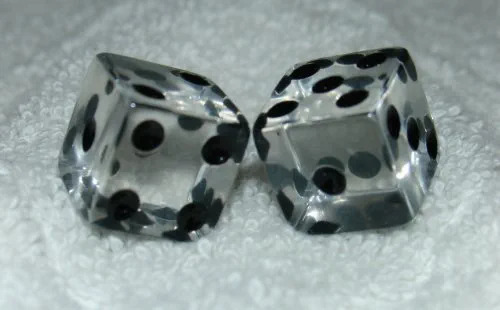
\includegraphics[scale=0.5]{dice.jpg} \\

Note: this image does not belong to me and was taken from an Amazon listing. \\
https://www.amazon.com/Vintage-Dice-Clear-Transparent-Pair/dp/B000UPTRIQ \\
The brand is called "Vintage Dice" and all rights belong to that entity. \\\\

The planned skybox is different from what is displayed in the image.
\end{document}
